\section{Gestionnaire des permissions}

Cette section décrit les actions de la page gestionnaire des permissions. Cette page n'est accessible qu'aux membre du staff qui sont admin.\newline

Cette page contient, à gauche, une liste des utilisateurs. À droite, l'utilisateur sélectionné y est affiché, avec des cases indiquant les permissions actuelles de cet utilisateur.

\begin{figure}[H]
\centering
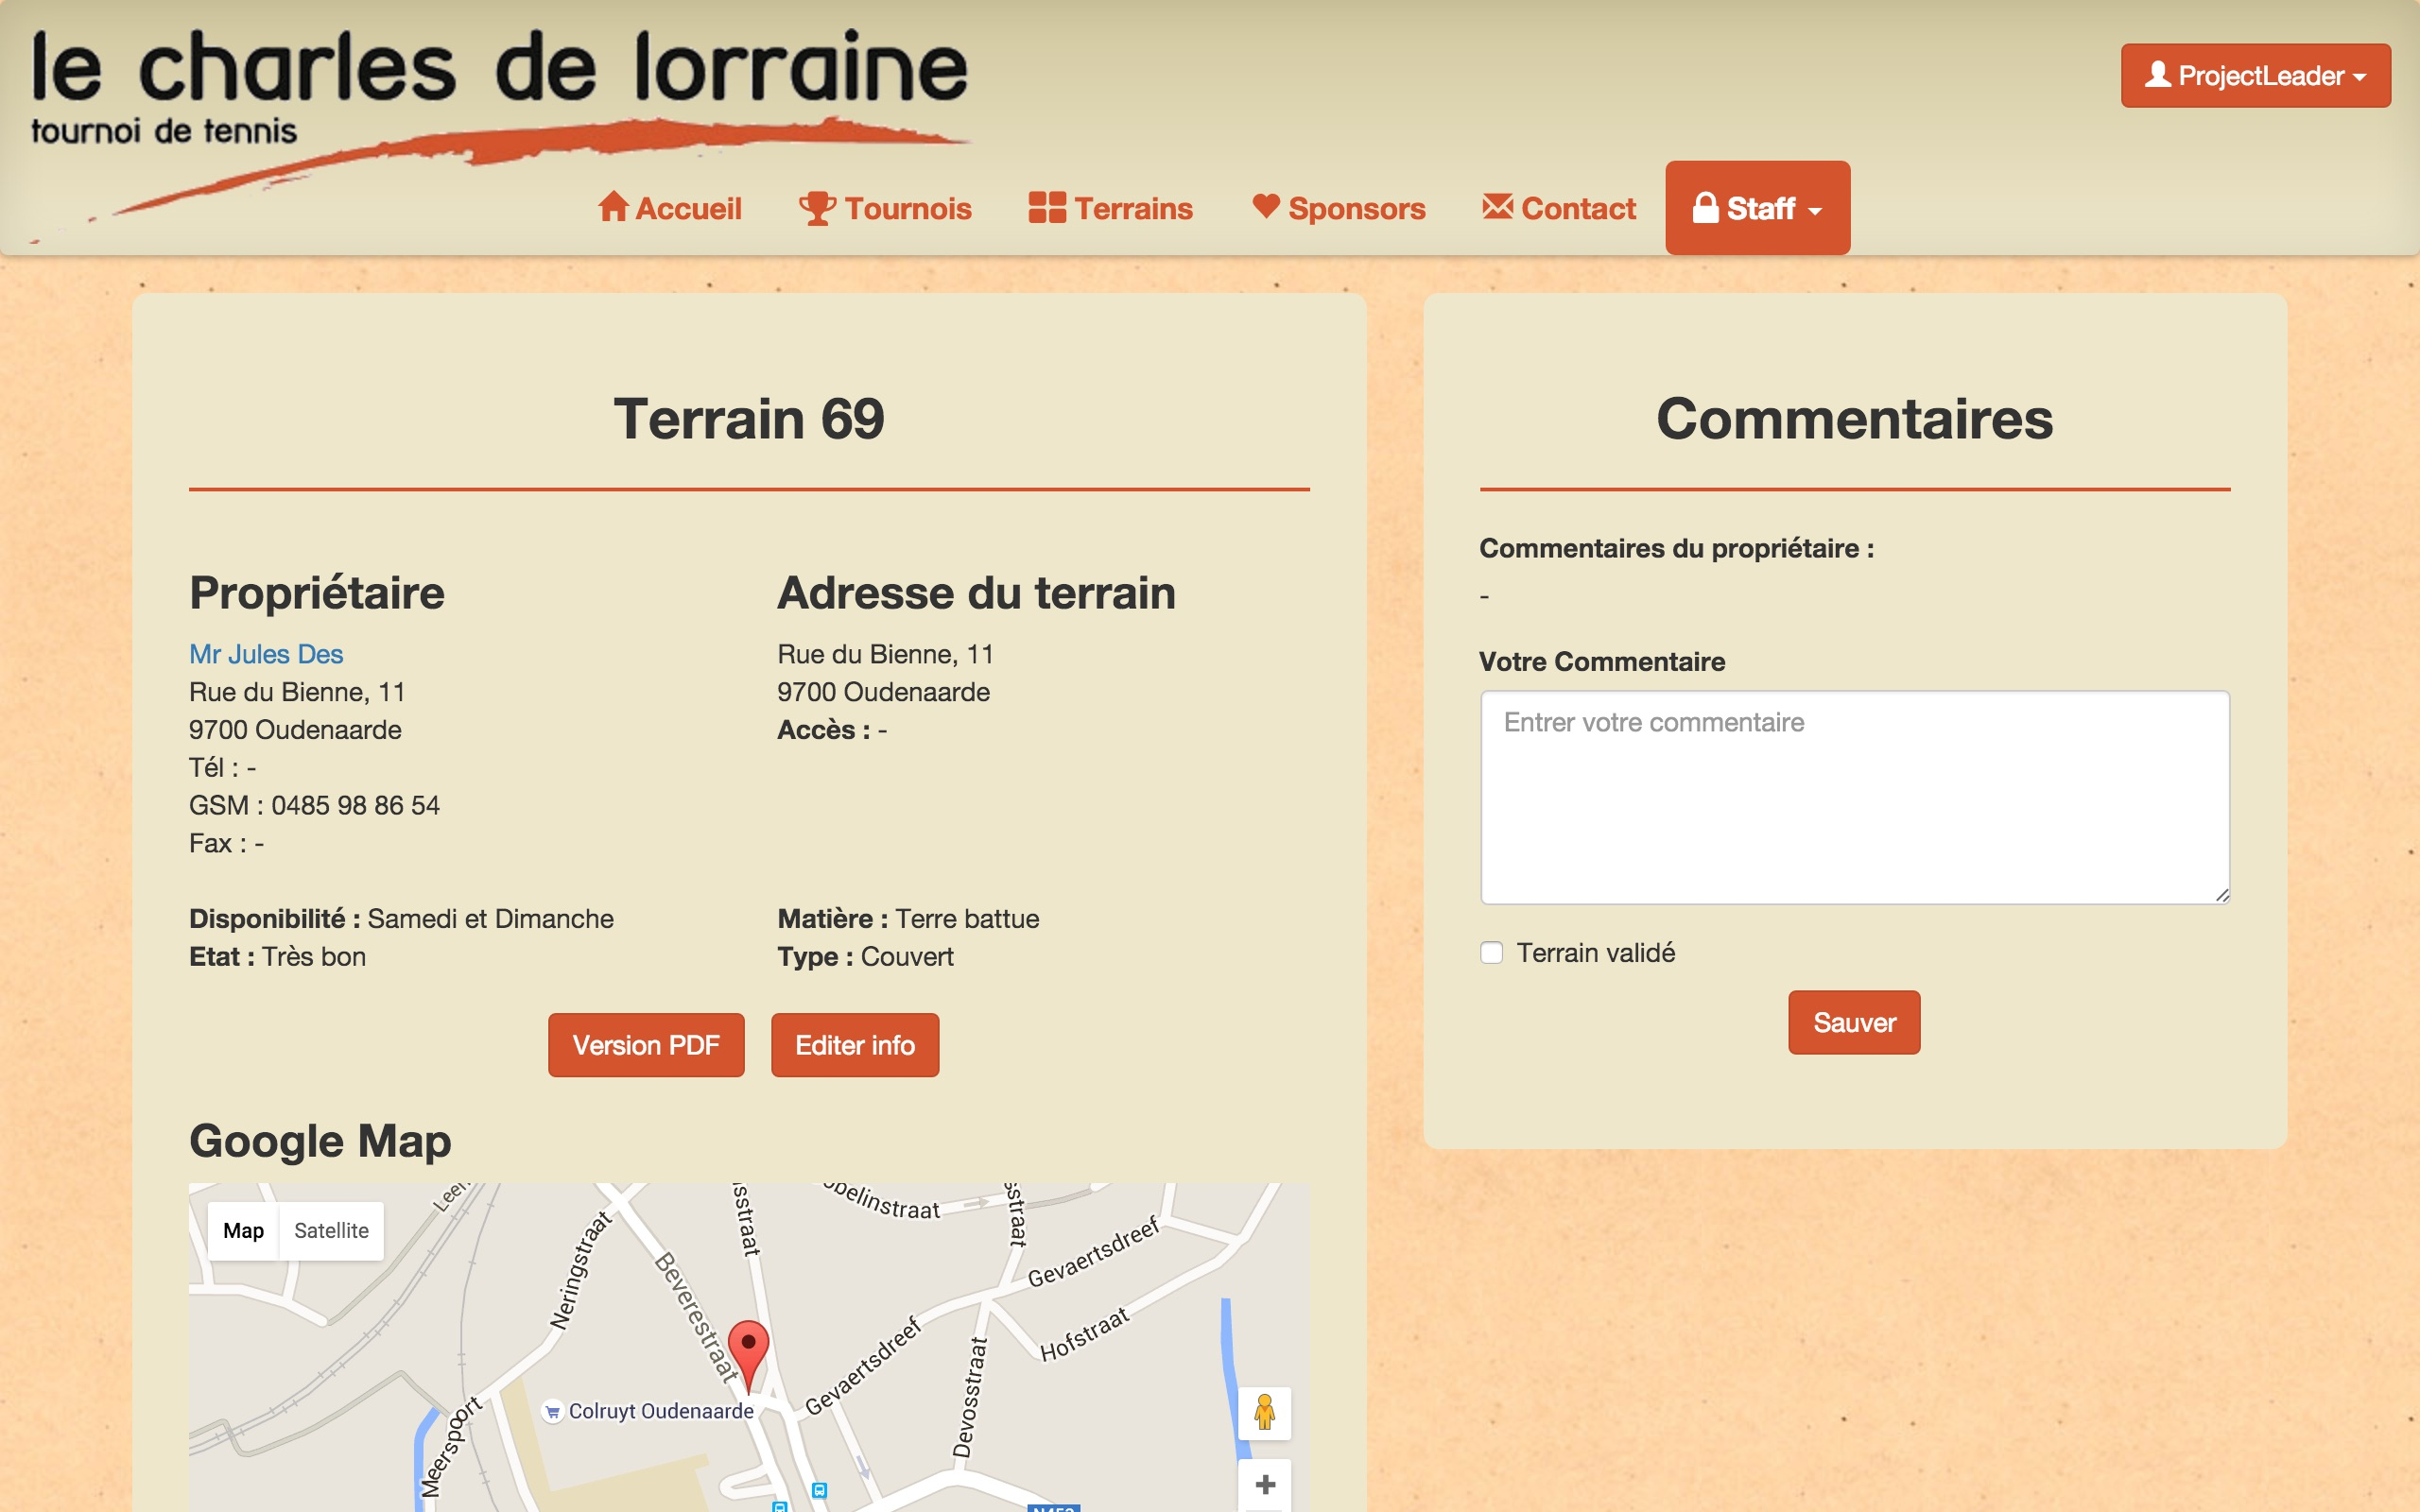
\includegraphics[scale=0.15]{user_images/staff/GererPermissions/001.jpg}
\caption{Gestionnaire des permissions}
\end{figure}

\subsection{Modifier les permissions d'un utilisateur}

Pour modifier les permission d'un utilisateur, il suffit d'abord de le sélectionner dans la liste des utilisateurs à gauche de la page.\newline

En sélectionnant un utilisateur (par exemple, le compte abab), et en cochant la case admin, l'utilisateur aura les droit admin dès qu'on aura cliqué sur le bouton "Valider".

\begin{figure}[H]
\centering
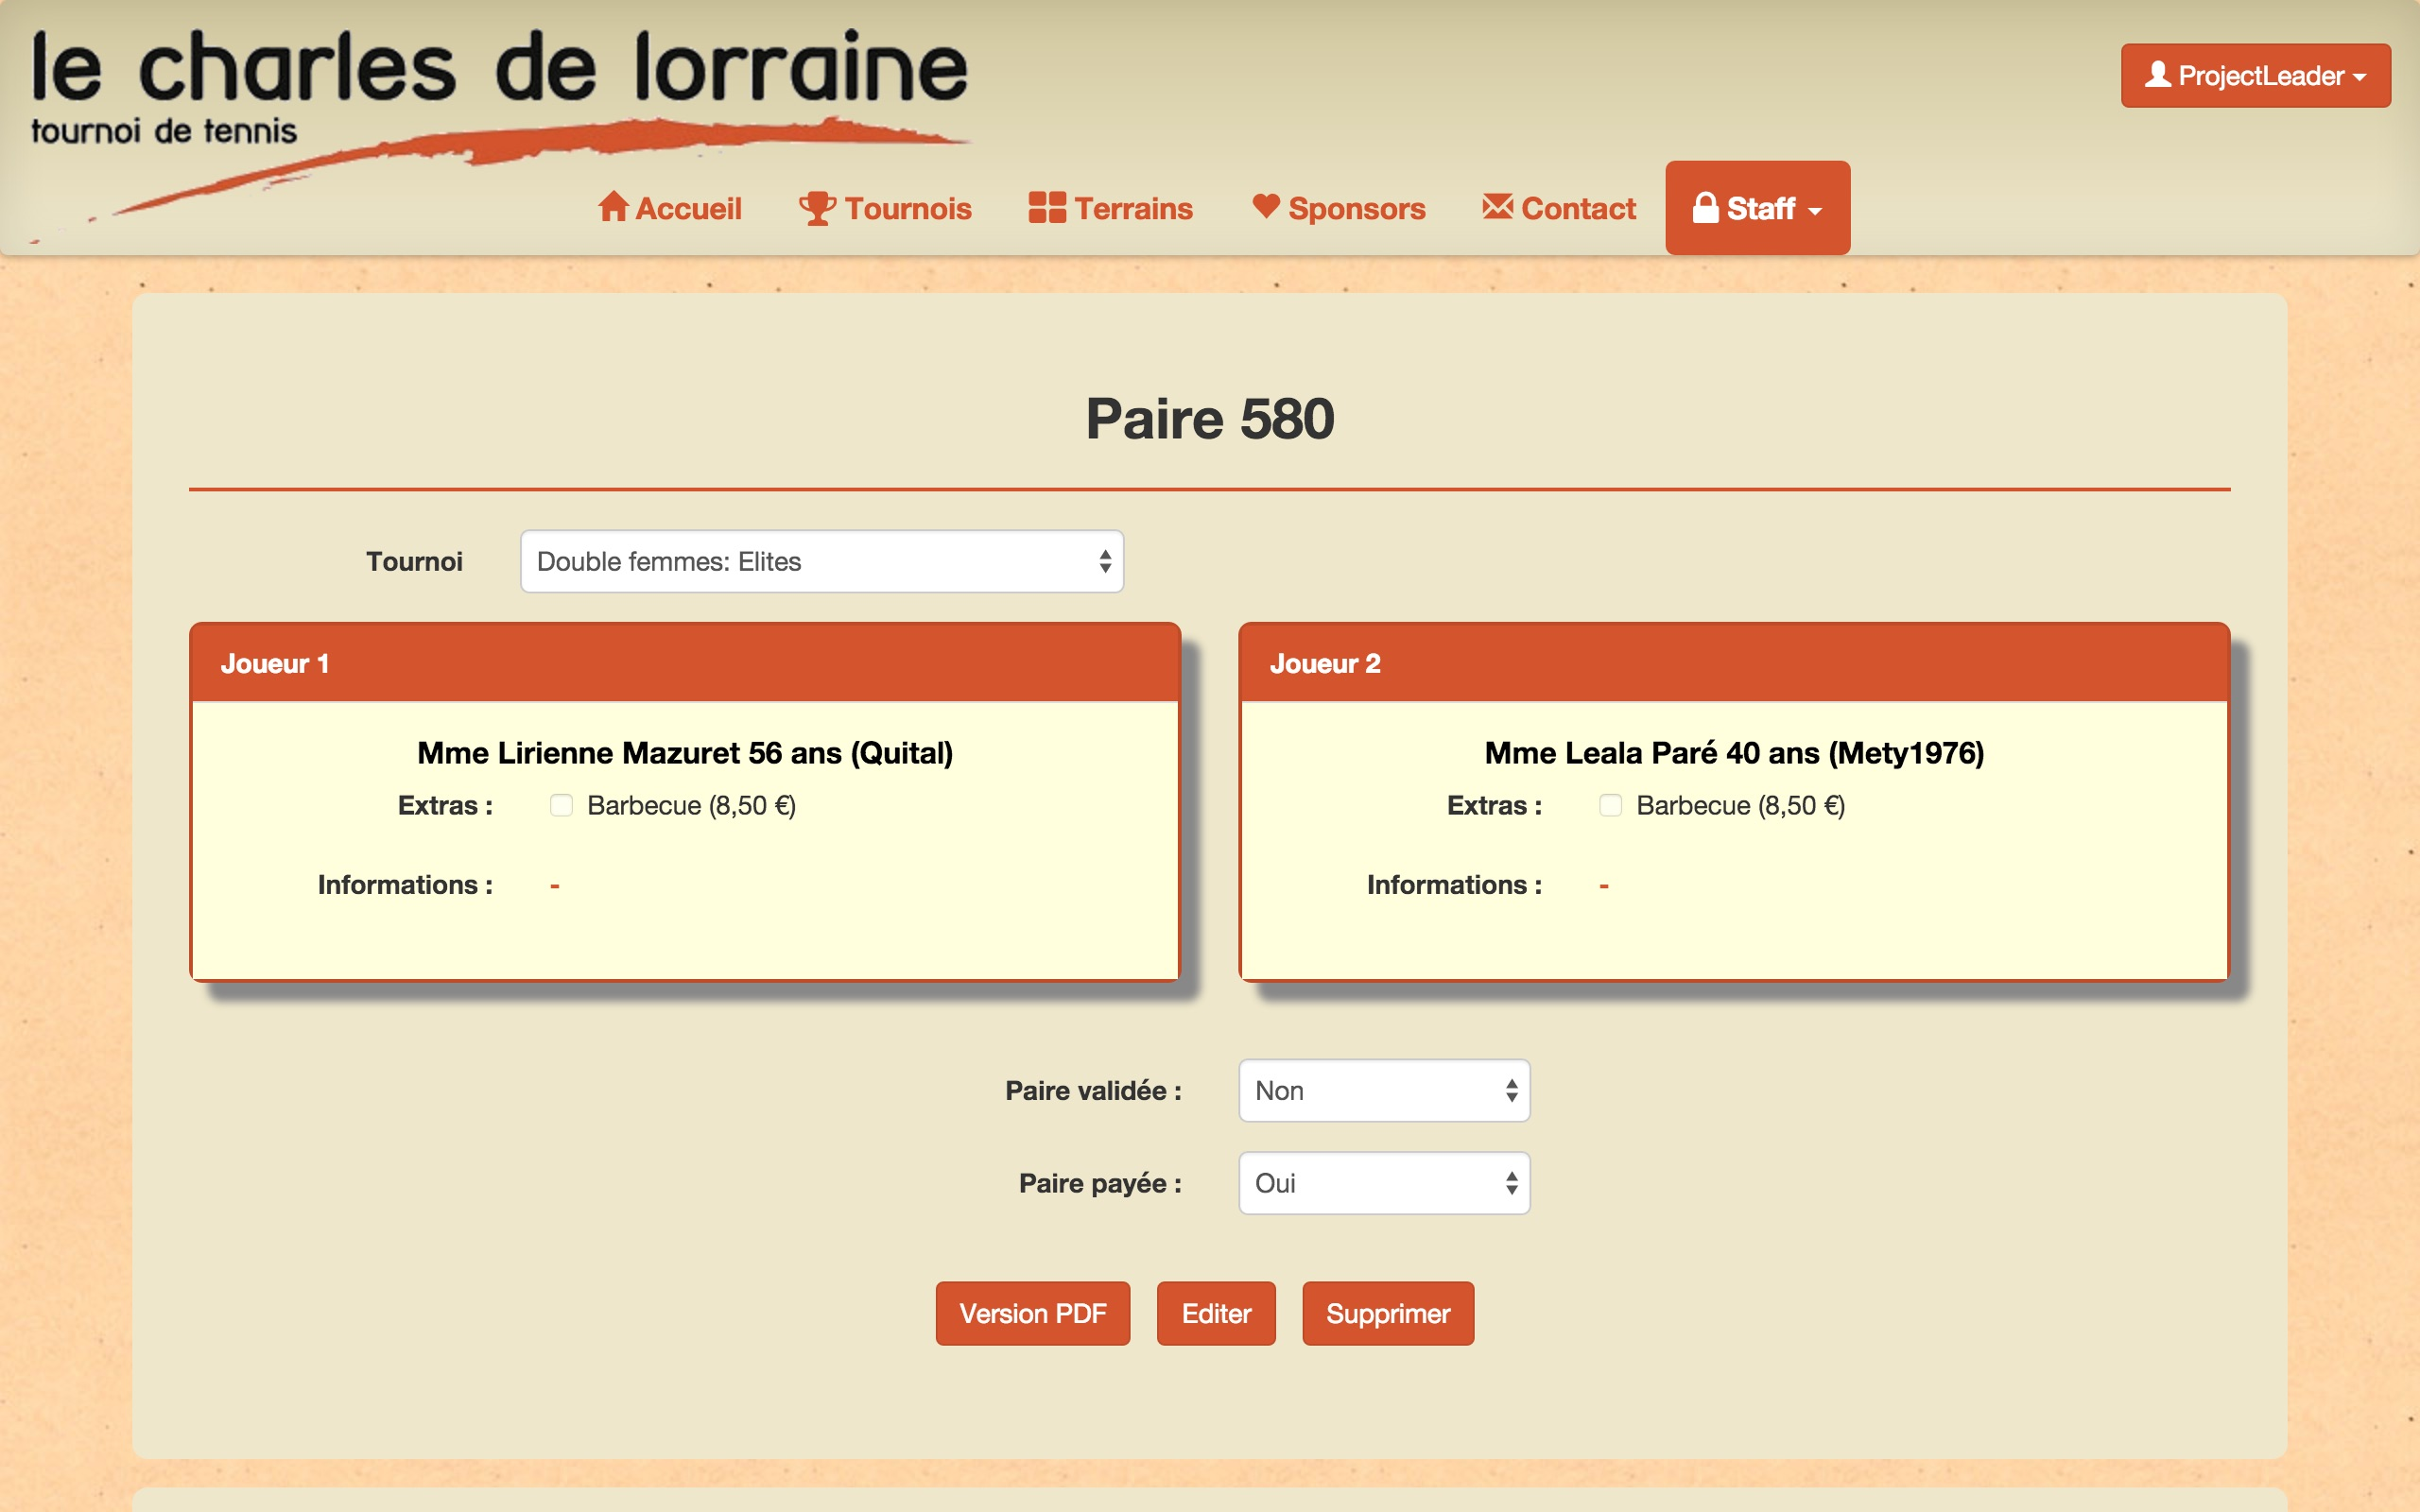
\includegraphics[scale=0.15]{user_images/staff/GererPermissions/002.jpg}
\caption{Ajout des permissions complet de staff à un utilisateur}
\end{figure}

Après validation des nouveaux droits de l'utilisateur abab, l'historique des modifications concernant les permissions indique clairement cette modification récente.

\begin{figure}[H]
\centering
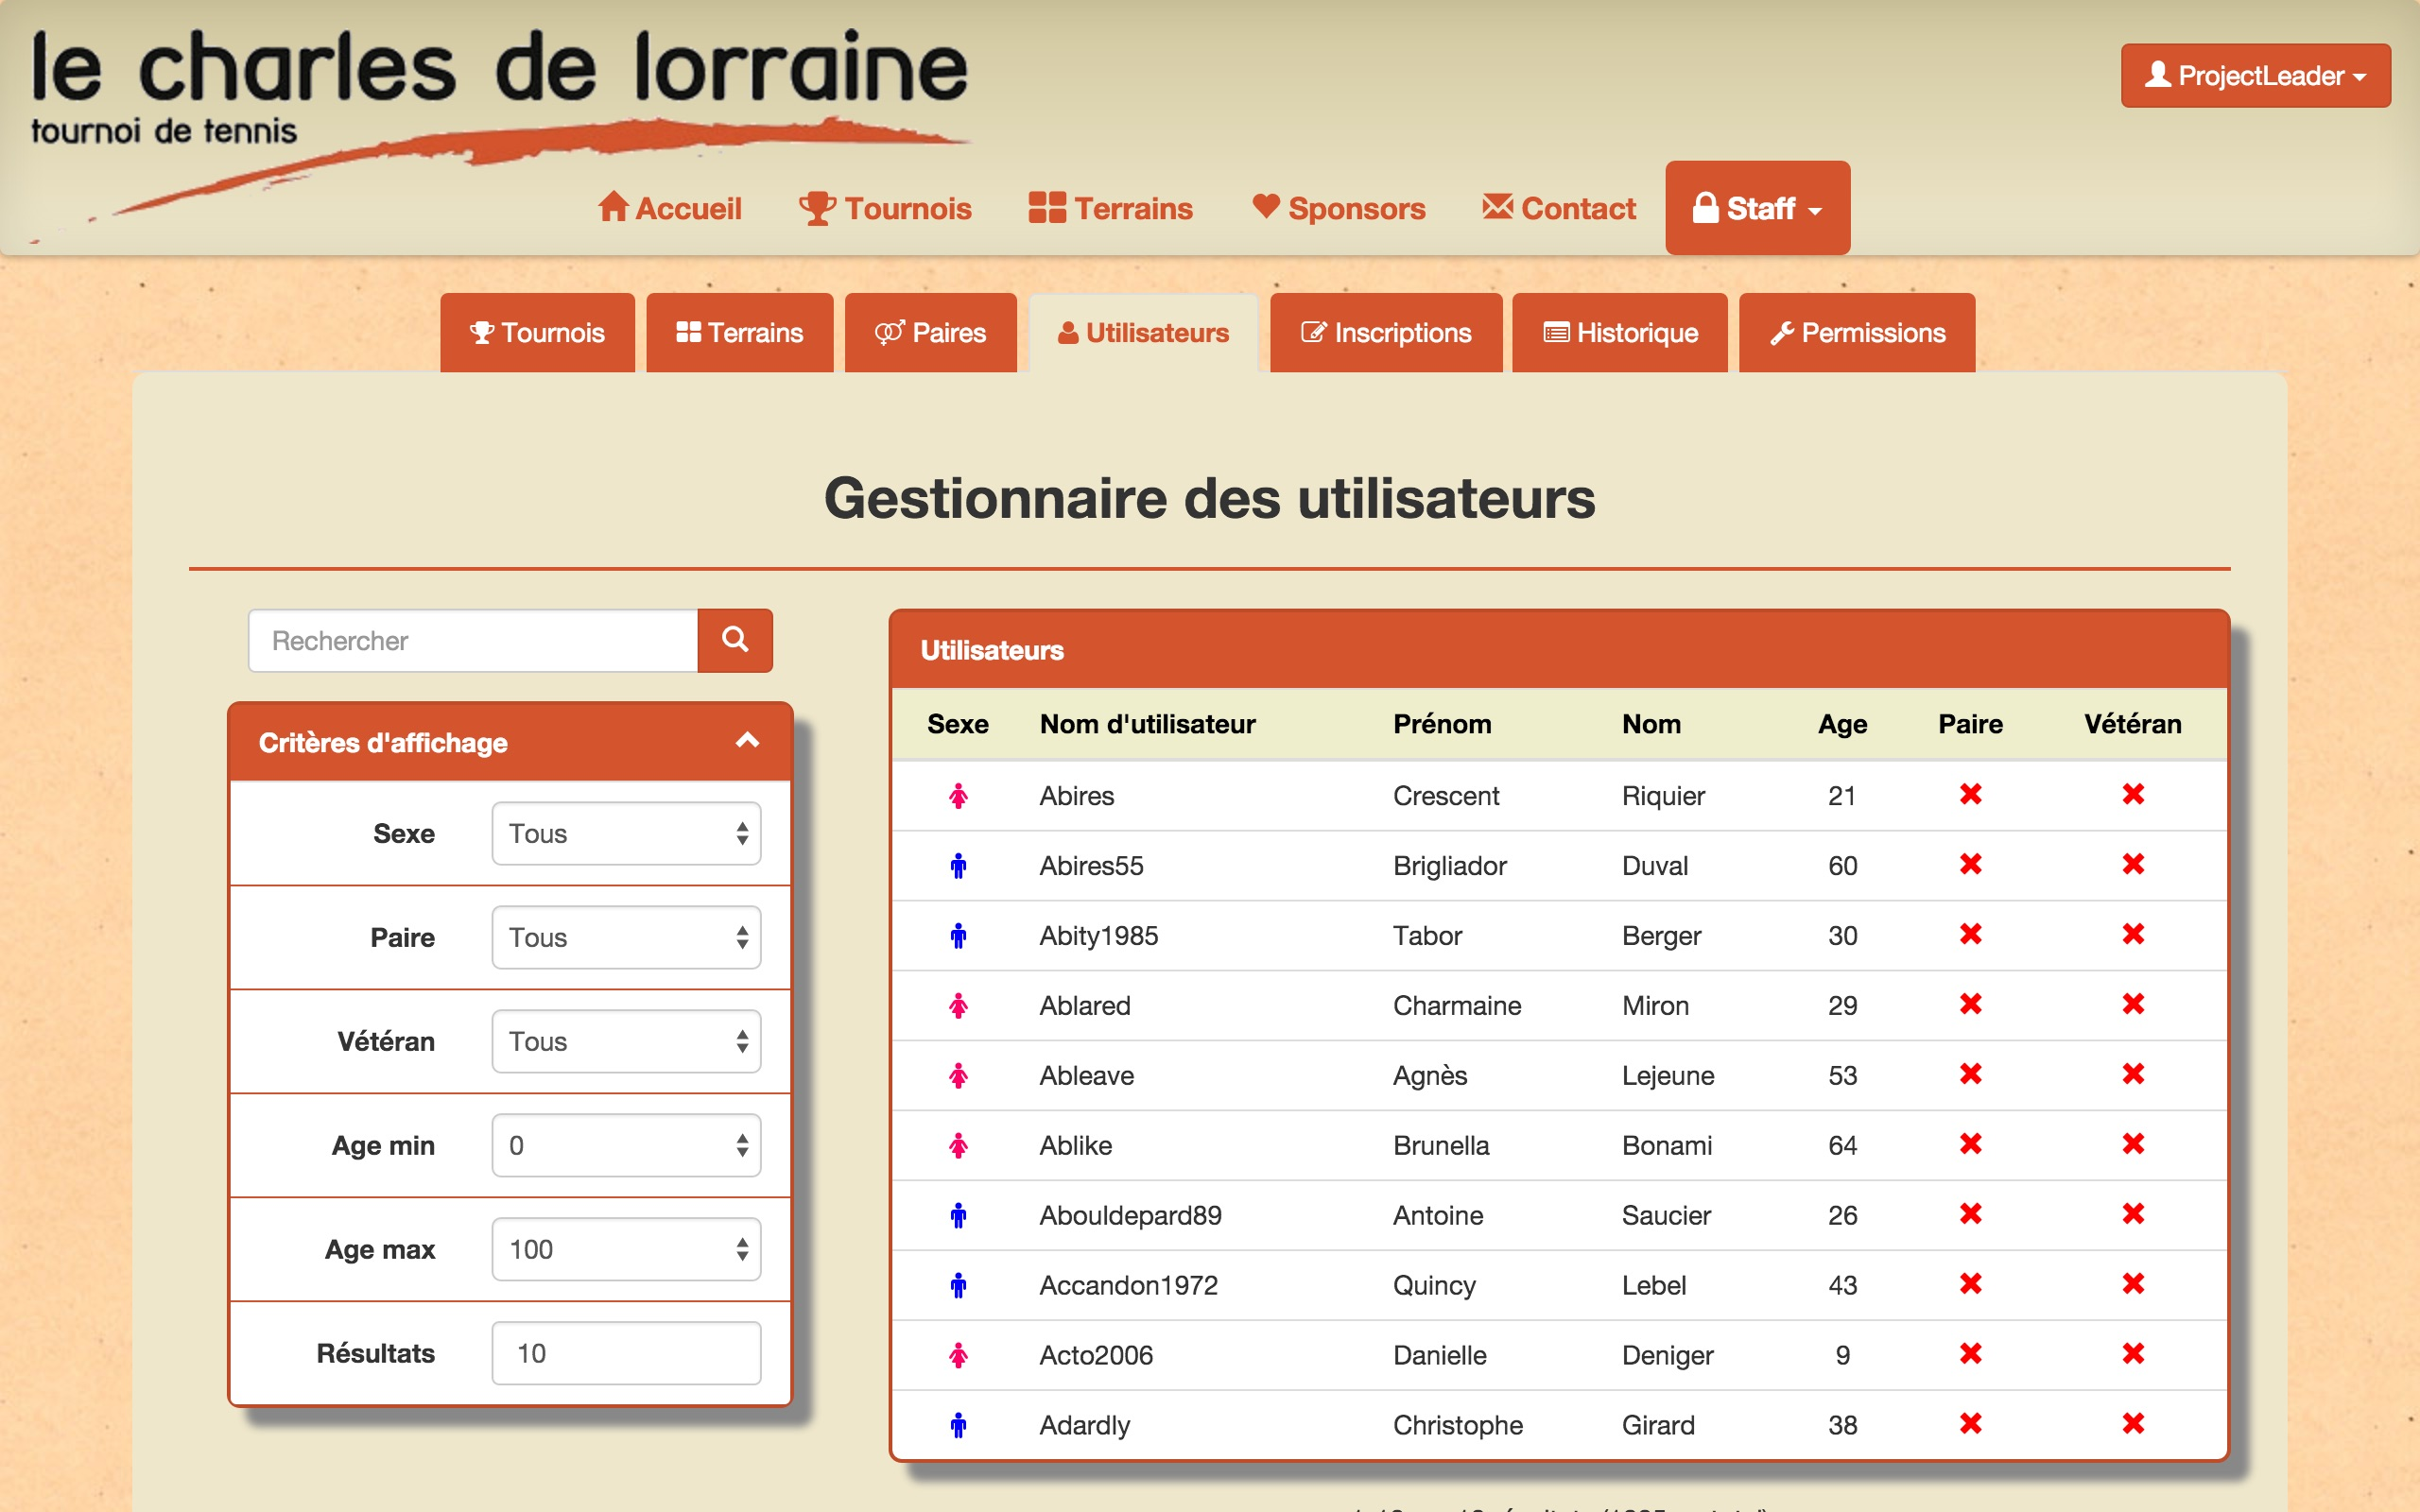
\includegraphics[scale=0.15]{user_images/staff/GererPermissions/003.jpg}
\caption{Permissions admin bien ajoutées}
\end{figure}

En se connectant avec l'utilisateur abab, on peut remarquer que toutes les pages staffs sont accessibles, alors qu'elles ne l'étaient avant l'octroi des droits admin.

\begin{figure}[H]
\centering
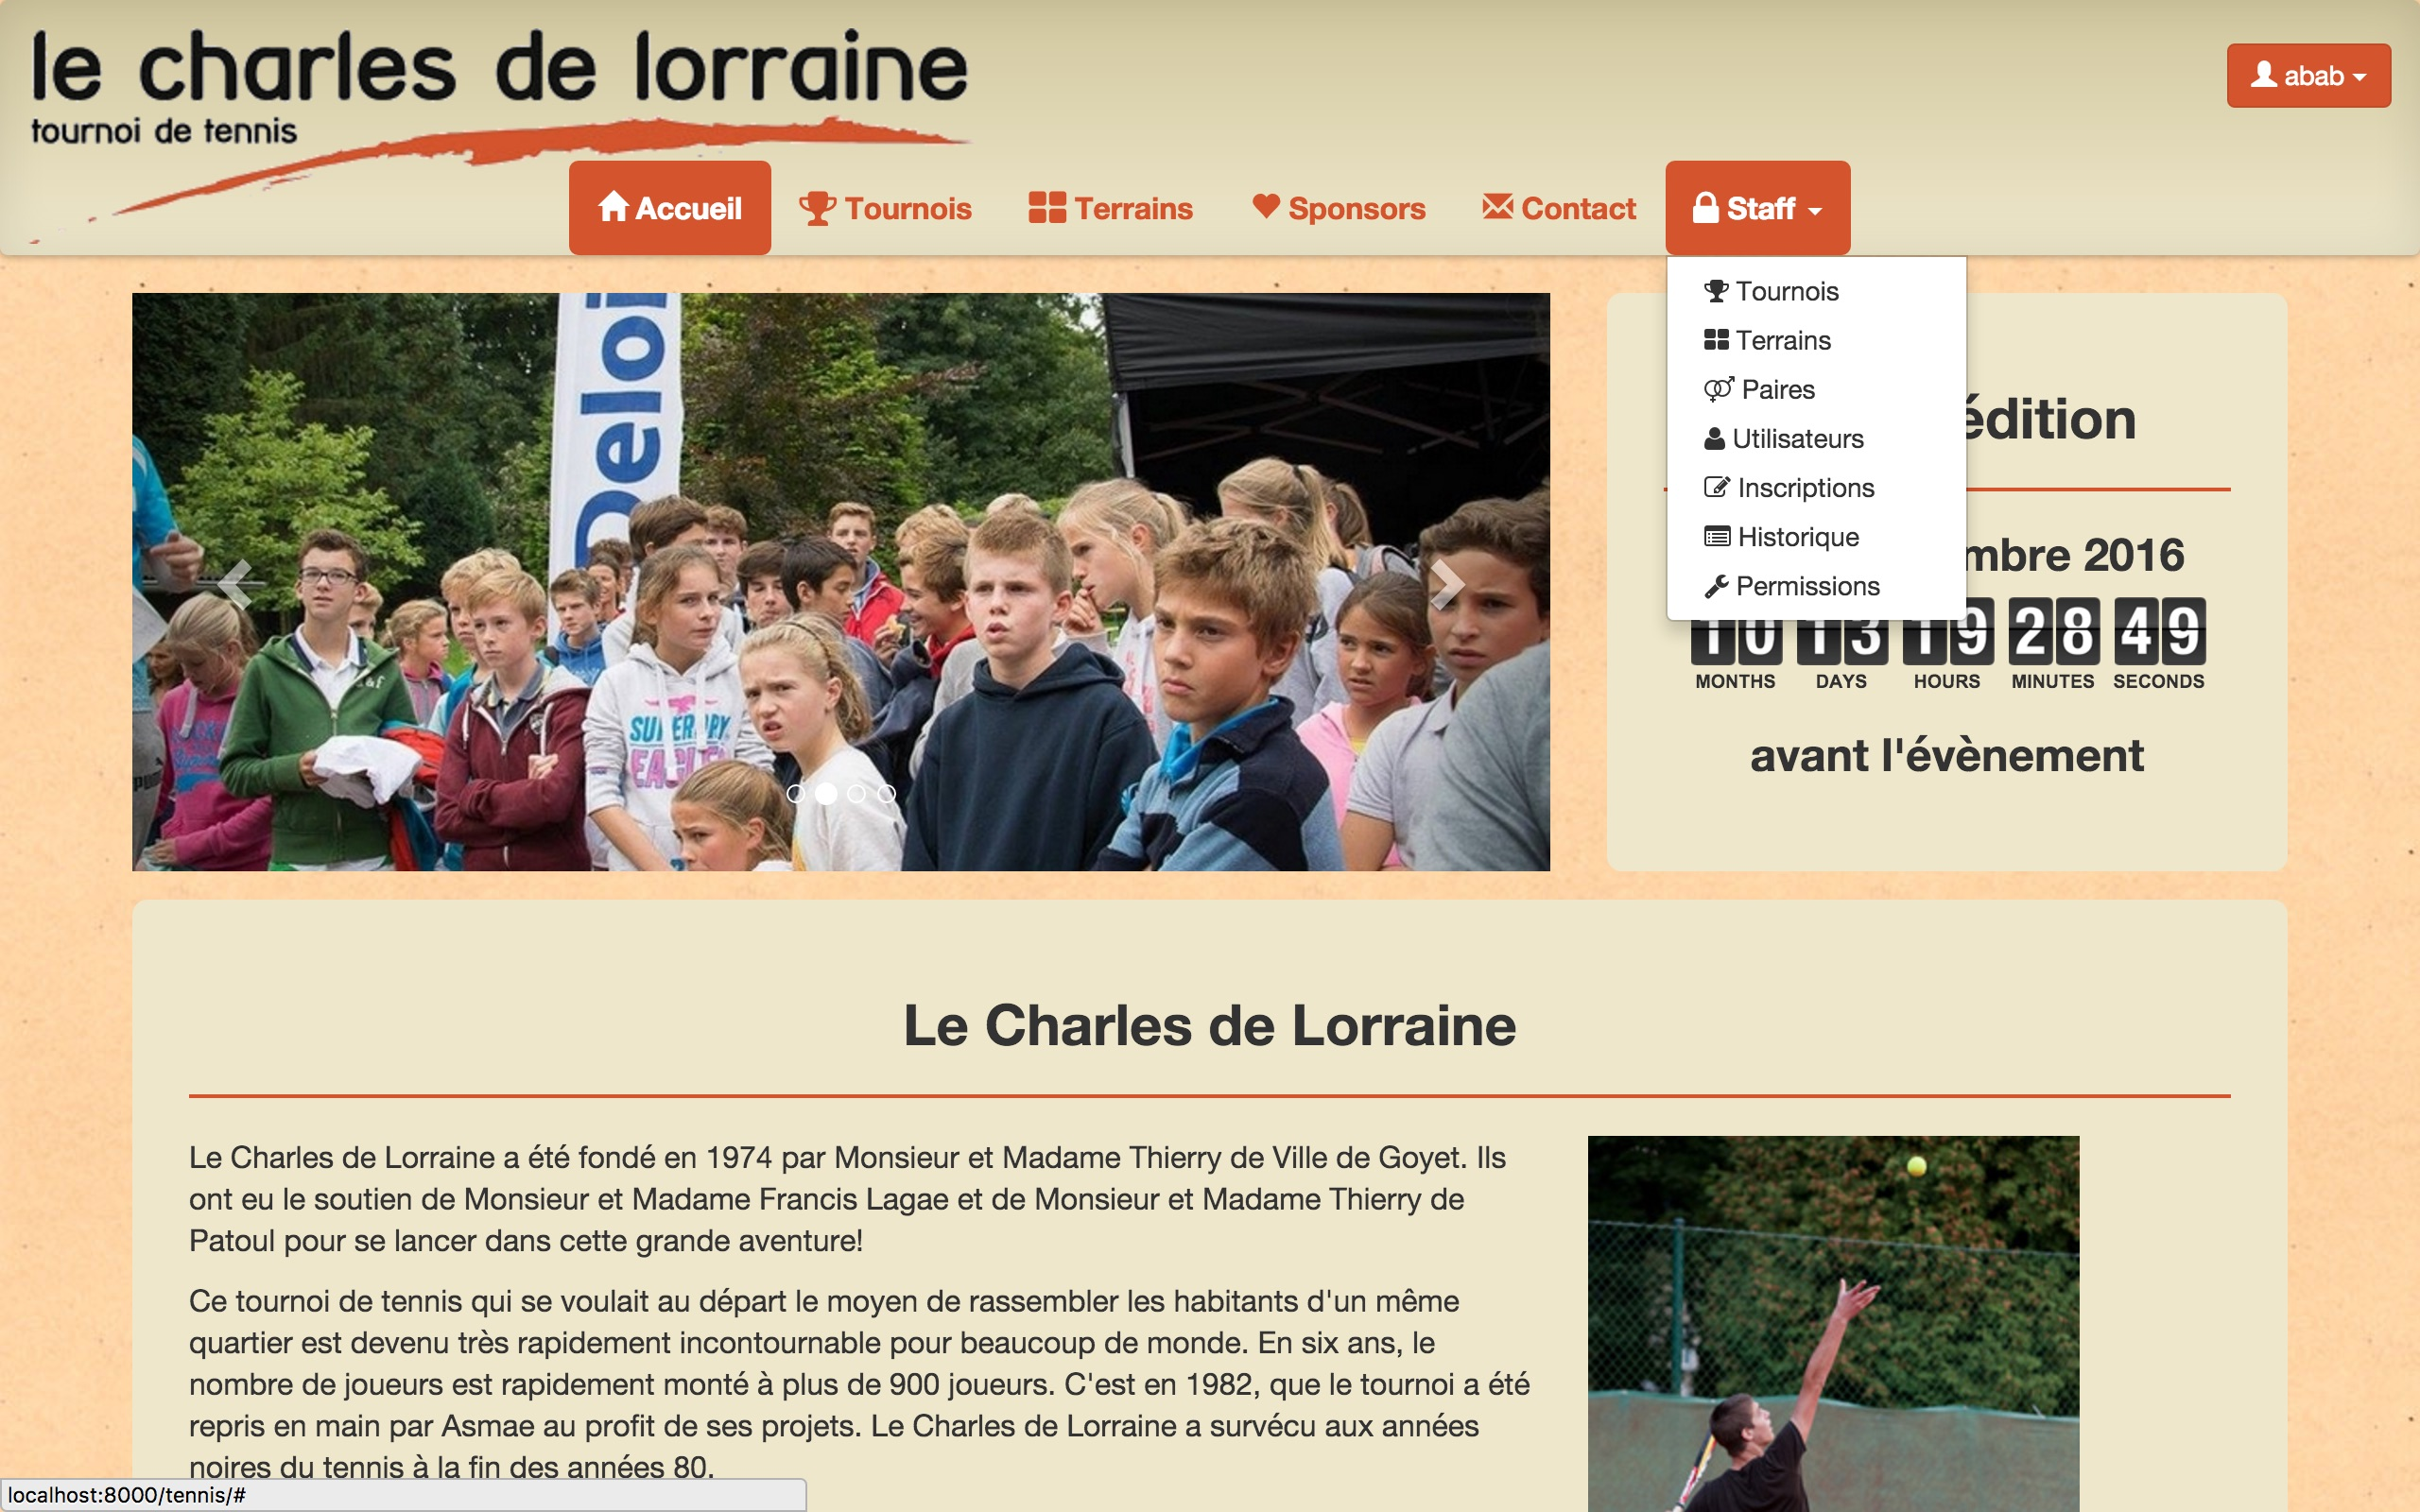
\includegraphics[scale=0.15]{user_images/staff/GererPermissions/004.jpg}
\caption{Accès aux partie staffs}
\end{figure}